% Chapter Template

\chapter{Control} % Main chapter title

\label{Chapter 3} % Change X to a consecutive number; for referencing this chapter elsewhere, use \ref{ChapterX}

\lhead{Chapter 3. \emph{Control}} % Change X to a consecutive number; this is for the header on each page - perhaps a shortened title

%
Once the simulation is fully implemented, the goal is to use it as a test-bench for different ways of controlling the structure. The second part of the project was fully consecrated on this part. PID (Proportional-Integrate-Derivative) control loops have been implemented to make sure that the command is respected by the creatures. Three different model were implemented and tested to control the creature: Fourier Decomposition, Central Pattern Generators and Liquid State Machines. The goal of each of these models is to represent the $\alpha_i(t)$ functions that are the angle of the joints with a vector of finite size. The Fourier Decomposition model for example (see Introduction) represent the angle functions with their Fourier Decomposition.

\begin{figure}[htbp]
    \centering
    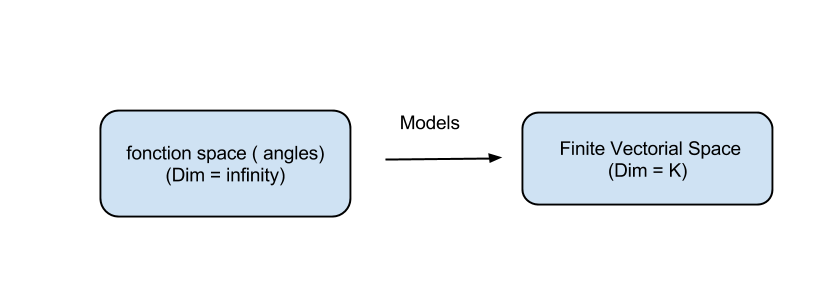
\includegraphics[scale=0.5]{Figures/models.png}
    \rule{35em}{0.5pt}
    \caption[Learning Model]{Learning Model}
    \label{fig:models}
\end{figure}

The two other models are described in this chapter.

\section{PID Control of the joints}

One of the problem to control accurately a joint is to adapt the command so that it can adapt to difficult situation. For instance, it is easier to walk in a swimming pool than on the ground and this is why people recovering after an injury do aquatic training. For a joint, it can be easy to do a movement in the air, but the same movement is more difficult when touching the ground. One way to avoid this problem is to implement PID (Proportional Integral Derivative) controller. This kind of controller is used in a lot of different situation in the world of automation to control degrees of freedom. In or case, servomotors often integrate such loops to account for these changes of use. In the simulation, at each step, the command of each degree of freedom of the structure is calculated using such a PID controller. 

\begin{figure}[htbp]
    \centering
    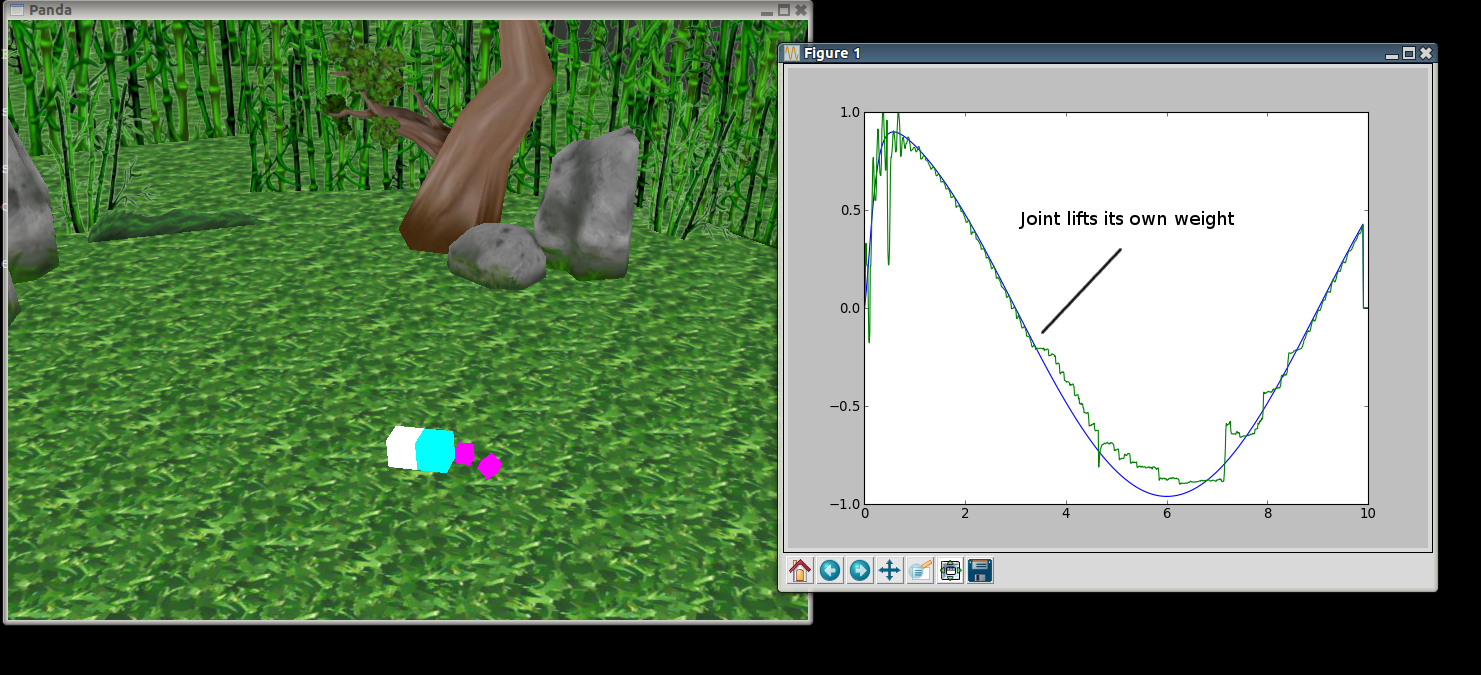
\includegraphics[scale=0.3]{Figures/servomotor.png}
    \rule{35em}{0.5pt}
    \caption[Answer of a joint to a sinusoidal command]{Answer of the joint to a sinusoidal command with PID Control}
    \label{fig:Snake}
\end{figure}

One of the problem with the control of the joints is the instability. On the simulation, as the angles have periodic values, if the joint has a high angle velocity, then between two steps, it can jump across the boundary and start turning faster and faster as the PID controller will not be able to work as well as if the degree of freedom were a linear parameter. The problem with this situation is that it can actually be seen as a good result for the learning algorithm, simply because the fitness function is the velocity of the creature. There are several things to prevent from this situation :

\begin{itemize}
    \item reduce the time between two steps of computation for the physics engine and the PID
    \item reduce the maximum torque available per joint
    \item punish the creature if the joints are moving to slow
    \item change the fitness function to maximise parameter under a certain energy level
\end{itemize}
        

Another issue is more a biological concern. The main goal of this project is to find solutions that are biologically inspired instead of using a classical automation approach (even though we can compare the elasticity of or muscles as such controllers\ldots). Therefore though the use of PID is necessary in many robotics applications, we will try to avoid using the in the second part of the project. 

\section{Central Pattern Generator}

Central Pattern Generators (CPGs) are neural networks, that can generate oscillation for the control of the muscles of or body. They are the consequence and the cause of the paradigm of periodic movement in the locomotion of animals. Different models have been implemented to represent CPGs. We can represent them as a graph of coupled oscillator, where each node influence the behaviour of its neighbours. For a first implementation I choose to test the model of CPG followed at EPFL (\cite{sproewitz}). 

The CPG Neural Network in that case, is a graph that follow the physical architecture of the robot, setting one node for each joint (hinge or vertebra) on the structure. The dynamic of the CPG is determined by a coupling weight matrix $w_{ij}$, a phase bias matrix between nodes $\varphi_{ij}$, the frequency of the different oscillator $\omega_i$ and the desired amplitude and offset of the oscillation. We can compute the angle using the following system of equation and an integration method (I used the Runge-Kutta method in this project)

\begin{equation*}
    \dot{\phi_i} = \omega_i + \sum{w_{ij} * r_j * sin(\phi_i - \phi_j - \varphi_{ij})} \tag{1}
\end{equation*}
\begin{equation*}
        \theta_i = x_i + r_i * cos(\phi_i)  \tag{2}
\end{equation*}
This two equation gives the angle of the oscillator ($\theta_i$) depending on the state variable of a node: $x_i$, $r_i$, $\phi_i$, that can be described respectively as the offset, the amplitude and the phase of the oscillator.

\begin{equation*}
    \acute{r_i} = ar(\frac ar (R_i - r_i) - \dot{r_i}) \tag{3}
\end{equation*}
\begin{equation*}
    \acute{x_i} = ax(\frac ax (X_i - x_i) - \dot{x_i}) \tag{4}
\end{equation*}

Equations (3) and (4) describe the dynamic of the amplitude and offset (a second order dynamic that converge to the desired values). This trick is to ensure continuity in the oscillations, even if some of the parameters of the oscillator change. $a_r$ and $a_x$ are gains to control the dynamic ($a_r = a_x = 20 rad/s$  \cite{sproewitz}). 


A modification of this model is possible to plug the measured value of the degrees of freedom. Instead of using the second order control loop on $\theta_i$ which is achieved with the PID, we can set this control on the phase. That way, if the joint has troubles achieving his movement, for instance when hitting the ground, the phase will be modified and the perturbation will have an impact on other joints through equation (1).

One way to do so is to add a term in the equation (1), with $\dot{\theta_{reali}}$ the measured angle velocity of the joint. 
\begin{equation*}
    \dot{\phi_i} = \omega_i + \sum{w_{ij} * r_j * sin(\phi_i - \phi_j - \varphi_{ij}) + a_{\phi} * \frac {\dot{\theta_{reali}} - \dot{\theta_i}} {r_i * sin (\phi_i)}} \tag{1}
\end{equation*}

If we derive (2) we get: 
\begin{equation*}
    \dot{\theta_i} = \dot{x_i} + \dot{r_i} * cos(\phi_i) + r_i * sin(\phi_i) * \dot{\phi_i} \tag{2'}
\end{equation*}

By making the assumption that the dynamic of the amplitude and the offset is slow compared to the phase, we get
\begin{equation*}
    \dot{\theta_i} = r_i * sin(\phi_i) * \dot{\phi_i} \tag{2''}
\end{equation*}
That way, if we consider small variation of the phase, we can deduce an error term on $\dot{\phi_i}$ from the error on $\dot{\theta_i}$ given by $\frac {\dot{\theta_{reali}} - \dot{\theta_i}} {r_i * sin (\phi_i)}$ that we can control with a gain ($a_{\phi}$).
For example if the movement of a joint is made difficult because of the ground, then the measured velocity of this joint will be smaller that expected. The consequence will be to accelerate the movement for this joint (the derivative of the phase will be bigger), but also for the other joints that are linked to this one. We can interpret this as neural communication in our body within the central pattern generator, but also as the elasticity between joints. For instance if achieving a movement is too difficult for a joint, using elasticity, it is possible to get help from joints that are near. 


\section{Liquid State Machine}

Liquid State Machine (LSM) and Echo State Network were independently and simultaneously introduced by Mass and al \cite{liquidstatemachine} and Jaeger and al. \cite{echostatejaeger} and present a way of generating oscillations \cite{echostate}. They were introduced as a way of using recurrent neural network for Machine learning purposes, as recurrent neural network are harder to train using the classical back-propagation algorithm. A LSM is created from a random recurrent neural network that contains N neurons and is called the reservoir. The state of the neurons in the reservoir are updated using the following equation: 
\begin{equation*}
    X_{t + 1} = f( W_r * X_{t})
\end{equation*}
 where $W_r$ is the random weight matrix inside the reservoir and f is the activation function ( in this project we used the hyperbolic tangent as the activation function)

Once this network is created, oscillations can be observed in the state of each neurons. A weight matrix is randomly initiated to produce linear combinations of these oscillations that can be plugged to control the joints angles of the creature.

\begin{equation*}
    \alpha_i(t) = \frac{\pi}{2} f( W_o * X_{t})
\end{equation*}

where $W_o$ is the output weights and f is also an activation function. We then multiply the results by $\frac{\pi}{2}$ to ensure that the angles are in an acceptable range for the control in any situation.

\begin{figure}[htbp]
    \centering
    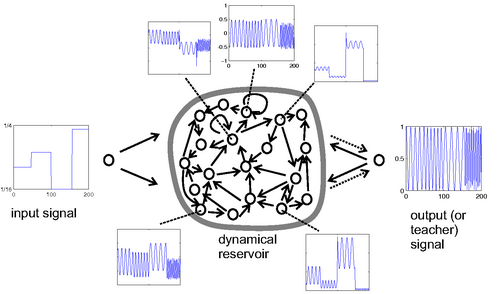
\includegraphics[scale=3.0]{Figures/echo_state.png}
    \rule{35em}{0.5pt}
    \caption[Liquid State Machine]{Liquid State Machine}
    \label{fig:echo_state}
\end{figure}


The idea of the Liquid State Machine is to focus the learning parameters on the output weights. The reservoir of neurons can be big, and produce a large variety of periodic signals. By learning the $W_o$ matrix ( of size $N * K$ where $N$ is the size of the reservoir and $K$ the number of hinge) each hinge can select some features of these oscillations. 

It is also possible to use a feedback loop in the network, by plugging the measured angles in the reservoir using the output weights. 

 



